
\section{\label{sec:polynomialLagrange}Polinom Lagrange}

Suatu fungsi yang grafiknya harus melalui sekumpulan titik yang ditentukan
disebut fungsi interpolasi\index{fungsi interpolasi}, dan kita mengatakan
bahwa fungsi tersebut menginterpolasi titik-titik yang ditentukan.
Selanjutnya, proses mencari fungsi semacam itu disebut interpolasi. 

Pada latihan \ref{polynomials}a di bagian \ref{sec:moreConvergenceDiagrams},
Anda diminta mencari polinom yang berakar di $-7,2$, dan $1\pm5i$
(dan tidak memiliki akar lain). Oleh karena itu, fungsi tersebut harus
berupa polinom dan grafiknya harus melalui titik-titik 
\begin{equation}
(-7,0),\ (2,0),\ (1+5i,0),\mbox{ dan }(1-5i,0).\label{eq:interpolationExample}
\end{equation}
Jika ditinjau kembali, pertanyaan itu dapat dirumuskan sebagai berikut:
carilah polinom yang melalui titik-titik \ref{eq:interpolationExample}
(dan tidak memiliki akar selain $-7$, $2$, $1+5i$, dan $1-5i$);
ini merupakan masalah interpolasi. Sekarang kita memperluas gagasan
ini dengan meninjau polinom yang grafiknya melalui titik-titik dengan
ordinat sembarang (bukan hanya $0$).

Kita mulai dari hal yang sudah dikenal. Polinom $p(x)=(x+7)(x-2)$
berakar di $-7$ dan $2$ sehingga grafiknya melalui $(-7,0)$ dan
$(2,0)$. Misalkan kita ingin mengubah $p$ agar grafiknya juga melalui
$(-1,1)$. Artinya, kita menginginkan $p(-7)=0$, $p(-1)=1$, dan
$p(2)=0$. Berangkat dari $p(x)=(x+7)(x-2)$, kita sudah mempunyai
$p(-7)=0$ dan $p(2)=0$, sehingga sebenarnya kita hanya perlu memusatkan
perhatian pada $p(-1)=1$. Dalam bentuknya sekarang, $p(-1)=(-1+7)(-1-2)=6(-3)=-18$,
sangat jauh dari $1$. Namun, $p(x)=(x+7)(x-2)$ bukan satu-satunya
polinom yang melalui $(-7,0)$ dan $(2,0)$. Ambil $a$ sembarang
bilangan real dan perhatikan bahwa $q(x)=a(x+7)(x-2)$ juga melalui
$(-7,0)$ dan $(2,0)$. Jika kita memilih $a$ sedemikian rupa sehingga
$q(-1)=1$, kita memperoleh fungsi yang diinginkan:
\[
q(-1)=a(-1+7)(-1-2)=-18a=1\Rightarrow a=-\frac{1}{18}.
\]
 $q(x)=-\frac{1}{18}(x+7)(x-2)$ melalui ketiga titik tersebut, yaitu
$(-7,0)$, $(2,0)$, dan $(-1,1)$. Namun, jangan sampai kita kehilangan
jejak asal konstruksi ini. $-\frac{1}{18}=\frac{1}{p(-1)}$, sehingga
sebenarnya fungsi yang diinginkan dapat ditulis sebagai $q(x)=\frac{p(x)}{p(-1)}$.
Memang, $q(-7)=\frac{p(-7)}{p(-1)}=0$, $q(2)=\frac{p(2)}{p(-1)}=0$,
dan $q(-1)=\frac{p(-1)}{p(-1)}=1$. 

Sekarang misalkan kita menginginkan polinom yang melalui $(-7,0)$,
$(2,0)$, dan $(-1,\sqrt{2})$. Seperti sebelumnya, kita mengetahui
bahwa $p(x)=(x+7)(x-2)$ mempunyai akar yang diinginkan dan $q(x)=\frac{p(x)}{p(-1)}$
memiliki sifat yang berguna, yaitu $q(-1)=1$. Kita menggunakan kedua
fakta ini untuk memperoleh jawaban. Bahkan, tanpa melakukan perhitungan
apa pun, kita mengetahui bahwa polinom 
\[
l(x)=\frac{p(x)}{p(-1)}\sqrt{2}
\]
adalah fungsi yang diinginkan. Luangkan waktu sejenak untuk memeriksa
bahwa $l(-7)=0$, $l(2)=0$, dan $l(-1)=\sqrt{2}$, dan memahami konstruksinya.
Gagasan ini merupakan benih dari apa yang disebut bentuk Lagrange
bagi polinom interpolasi.

Kini kita siap membiarkan ordinatnya sembarang! Misalkan kita menginginkan
polinom yang melalui $(-7,y_{1}),$ $(2,y_{2})$, dan $(-1,y_{3})$.
Kita mengetahui bahwa polinom $p_{3}(x)=(x+7)(x-2)$ berakar di $-7$
dan $2$, sehingga polinom $l_{3}(x)=\frac{p_{3}(x)}{p_{3}(-1)}y_{3}$
bernilai nol di $-7$ dan $2$, sedangkan $l_{3}(-1)=y_{3}$. Ini
merupakan langkah pertama yang baik. Polinom ini menghasilkan ordinat
yang tepat pada $-1$ dan bernilai nol di $-7$ dan $2$. Dengan cara
serupa, kita dapat mengonstruksi polinom $p_{2}(x)=(x+7)(x+1)$ yang
berakar di $-7$ dan $-1$; dari polinom ini kita dapat mengonstruksi
polinom $l_{2}(x)=\frac{p_{2}(x)}{p_{2}(2)}y_{2}$ yang bernilai nol
di $-7$ dan $-1$, sedangkan $l_{2}(2)=y_{2}$. Ini merupakan langkah
kedua yang baik. Polinom ini menghasilkan ordinat yang tepat pada
$2$ dan bernilai nol di $-7$ dan $-1$. Sekarang tinjau jumlah $(l_{3}+l_{2})$.
$l_{3}(-1)=y_{3}$ dan $l_{2}(-1)=0$, sehingga $(l_{3}+l_{2})(-1)=y_{3}$.
Dengan cara serupa, $l_{3}(2)=0$ dan $l_{2}(2)=y_{2}$, sehingga
$(l_{3}+l_{2})(2)=y_{2}$. Selain itu, $(l_{3}+l_{2})(-7)=0$. Kini
kita mempunyai polinom yang melalui dua dari tiga titik yang disyaratkan
dan bernilai nol pada absis titik ketiga. Jika kita mempunyai polinom
yang menghasilkan ordinat yang tepat pada $-7$ dan bernilai nol di
$2$ dan $-1$, kita dapat menambahkannya ke jumlah tersebut dan menyelesaikan
konstruksi. Namun, justru polinom seperti inilah yang telah kita konstruksikan!
Kita menetapkan $p_{1}(x)=(x+1)(x-2)$ dan $l_{1}(x)=\frac{p_{1}(x)}{p_{1}(-7)}y_{1}$,
lalu memperhatikan bahwa $l_{1}$ menghasilkan ordinat yang tepat
pada $-7$ dan bernilai nol di $2$ dan $-1$, tepat seperti yang
kita perlukan. Akhirnya, polinom yang diinginkan adalah $(l_{1}+l_{2}+l_{3})$.
Tabel \ref{tab:interpolationExample} 
\begin{table}
\hrule \caption{\label{tab:interpolationExample}Polinom yang melalui $(-7,y_{1})$,
$(2,y_{2})$, dan $(-1,y_{3})$.}

\centering{}\medskip{}
\begin{tabular}{c|ccc|c}
$x$ & $l_{1}(x)=\frac{p_{1}(x)}{p_{1}(-7)}y_{1}$ & $l_{2}(x)=\frac{p_{2}(x)}{p_{2}(2)}y_{2}$ & $l_{3}(x)=\frac{p_{3}(x)}{p_{3}(-1)}y_{3}$ & $(l_{1}+l_{2}+l_{3})(x)$\tabularnewline
\hline 
$-7$ & $y_{1}$ & $0$ & $0$ & $y_{1}$\tabularnewline
$2$ & $0$ & $y_{2}$ & $0$ & $y_{2}$\tabularnewline
$-1$ & $0$ & $0$ & $y_{3}$ & $y_{3}$\tabularnewline
\end{tabular}\medskip{}
\hrule 
\end{table}
merangkum konstruksi tersebut.

Sekarang kita siap melakukan generalisasi sepenuhnya. Misalkan $n\geq1$
dan $x_{0},x_{1},\ldots,x_{n}$ adalah $n$ bilangan real yang berbeda.
Kita menggunakan notasi $P_{n}(x)$ untuk polinom berderajat terendah
yang menginterpolasi titik-titik
\[
(x_{0},y_{0}),(x_{1},y_{1}),\ldots,(x_{n},y_{n}).
\]

Dengan menetapkan ${\displaystyle p_{i}(x)=\prod_{\substack{j=0\\
j\neq i
}
}^{n}(x-x_{j})=(x-x_{0})\cdots(x-x_{i-1})(x-x_{i+1})\cdots(x-x_{n})}$, salah satu rumus untuk $P_{n}$ adalah 
\begin{equation}
L_{n}(x)=\sum_{i=0}^{n}\frac{p_{i}(x)}{p_{i}(x_{i})}y_{i}.\label{eq:lagrangeInterpolatingPolynomial}
\end{equation}
Dalam bentuk ini, $L_{n}$ disebut \textit{bentuk Lagrange}\index{bentuk Lagrange}
dari $P_{n}$. Demi keringkasan, bentuk ini sering disebut polinom
interpolasi Lagrange, atau bahkan polinom Lagrange. Namun, apa pun
namanya, polinom interpolasi berderajat terendah itu tetaplah $P_{n}$.
Kita akan tetap menyebutnya polinom interpolasi berderajat terendah,
atau menggunakan notasi $P_{n}$, jika bentuknya tidak penting; dan
kita akan menambahkan frasa \textit{bentuk Lagrange}, atau menggunakan
notasi $L_{n}$, jika bentuknya penting.

Penggunaan utama polinom interpolasi dalam analisis numerik adalah
untuk menghampiri fungsi nonpolinom dengan cara berikut. Misalkan
kita mengetahui nilai $f$ pada beberapa titik. Artinya, kita mengetahui
$f(x_{0})=y_{0},f(x_{1})=x_{1},\ldots,f(x_{n})=y_{n}$ dan mungkin
tidak mengetahui banyak hal lainnya. Berdasarkan konstruksinya, polinom
interpolasi berderajat terendah yang melalui $n+1$ titik
\[
(x_{0},y_{0}),(x_{1},y_{1}),\ldots,(x_{n},y_{n})
\]
akan sama dengan $f$ pada $x_{0},x_{1},\ldots,x_{n}$ dan kita dapat
menyatakan dengan cukup tepat seberapa dekat polinom interpolasi ini
dengan $f$ pada titik-titik lain. Nilai polinom interpolasi pada
``titik-titik lain'' inilah yang kita sebut hampiran terhadap fungsi
nonpolinom.

Dengan menetapkan $a=\min(x_{0},\ldots,x_{n},x)$ dan $b=\max(x_{0},\ldots,x_{n},x)$,
kita memperoleh hasil berikut. Jika $f$ mempunyai $n+1$ turunan
pada $(a,b)$ dan $f,f',f'',\ldots,f^{(n)}$ semuanya kontinu pada
$[a,b]$, maka terdapat $\xi_{x}\in(a,b)$ sedemikian sehingga 
\begin{equation}
f(x)-P_{n}(x)=\frac{f^{(n+1)}(\xi_{x})}{(n+1)!}(x-x_{0})(x-x_{1})\cdots(x-x_{n}).\label{eq:lagrangeInterpolatingPolynomialError}
\end{equation}
Menariknya, hasil ini dibuktikan dengan meninjau bentuk Lagrange dari
suatu polinom interpolasi dalam variabel $t$ yang sama dengan galat
pada $x$ dan sama dengan nol pada setiap $x_{i}$. Polinom itu adalah
\[
\Lambda(t)=\left[P_{n}(x)-f(x)\right]\frac{(t-x_{0})(t-x_{1})\cdots(t-x_{n})}{(x-x_{0})(x-x_{1})\cdots(x-x_{n})}.
\]

\noindent\begin{digression}{$\Lambda$} 

\noindent$\Lambda$ adalah huruf kapital kesebelas dalam alfabet
Yunani dan dilafalkan  \texttt{\textbf{lam}}\texttt{-}\texttt{\textit{da}}.
Bentuk huruf kecilnya, $\lambda$, jauh lebih sering muncul dalam
matematika dan kerap menyatakan nilai eigen.

\noindent\end{digression} 

\noindent Dengan mengurangkan polinom ini dari galat, $e(t)=P_{n}(t)-f(t)$,
kita memperoleh fungsi
\[
g(t)=e(t)-\Lambda(t),
\]
yang bernilai nol untuk semua $t=x_{0},x_{1},\ldots,x_{n},x$. Karena
$g,g',\ldots,g^{(n)}$ semuanya kontinu pada $[a,b]$ dan $g^{(n+1)}$
ada pada $(a,b)$, berdasarkan Teorema Rolle yang Diperumum terdapat
$\xi_{x}\in(a,b)$ sedemikian sehingga $g^{(n+1)}(\xi_{x})=0$. Di
sisi lain, 
\begin{eqnarray*}
g^{(n+1)}(\xi_{x}) & = & e^{(n+1)}(\xi_{x})-\Lambda^{(n+1)}(\xi_{x})\\
 & = & P_{n}^{(n+1)}(\xi_{x})-f^{(n+1)}(\xi_{x})-\Lambda^{(n+1)}(\xi_{x}),
\end{eqnarray*}
dan $P_{n}$ merupakan polinom berderajat paling tinggi $n$. Oleh
karena itu, $P_{n}^{(n+1)}(t)=0$ untuk setiap $t$ dan kita memperoleh
$g^{(n+1)}(\xi_{x})=-f^{(n+1)}(\xi_{x})-\Lambda^{(n+1)}(\xi_{x})=0$.
Akibatnya, 
\[
f^{(n+1)}(\xi_{x})=-\Lambda^{(n+1)}(\xi_{x}).
\]
Namun, $\Lambda$ adalah polinom berderajat $n+1$ dalam $t$, sehingga
turunan ke-$(n+1)$ terhadap $t$ konstan terhadap $t$. Kita menuliskan
$\Lambda$ sebagai
\[
\Lambda(t)=\frac{P_{n}(x)-f(x)}{(x-x_{0})(x-x_{1})\cdots(x-x_{n})}\left[t^{n+1}+b_{n}t^{n}+\cdots+b_{0}t^{0}\right]
\]
untuk beberapa konstanta $b_{n},b_{n-1},\ldots,b_{0}$, dan akibatnya,
\[
\Lambda^{(n+1)}(t)=\frac{P_{n}(x)-f(x)}{(x-x_{0})(x-x_{1})\cdots(x-x_{n})}\cdot(n+1)!,
\]
dengan substitusi kita memperoleh
\[
f^{(n+1)}(\xi_{x})=\frac{f(x)-P_{n}(x)}{(x-x_{0})(x-x_{1})\cdots(x-x_{n})}\cdot(n+1)!
\]
atau, secara ekuivalen,
\[
\frac{f^{(n+1)}(\xi)}{(n+1)!}(x-x_{0})(x-x_{1})\cdots(x-x_{n})=f(x)-P_{n}(x)
\]
seperti yang hendak dibuktikan.

Gambar \ref{fig:Three-interpolating-functions.} 
\begin{figure}
\caption{\label{fig:Three-interpolating-functions.}Tiga fungsi yang diinterpolasi.
Dari atas ke bawah, $e^{\sin\left((x+1)^{2}\right)}$, $\sin\left(e^{(x+1)^{2}}\right)$,
dan fungsi fraktal sebagaimana didefinisikan pada bagian \ref{sec:rootFindingChallenge}.
$f$ ditampilkan dengan warna hitam, sedangkan interpolannya, $L_{6}$,
dengan warna merah.}

\centering{}%
\begin{tabular}{cc}
$f(x)$ dan $L_{6}(x)$ & $f^{(6)}(x)$\tabularnewline
\hline 
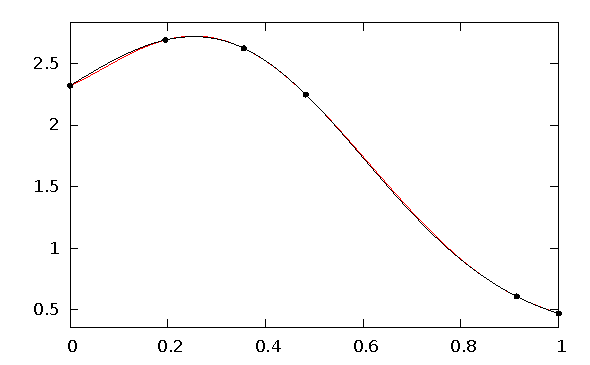
\includegraphics[scale=0.75]{figures/interpolation-polynomials1} & 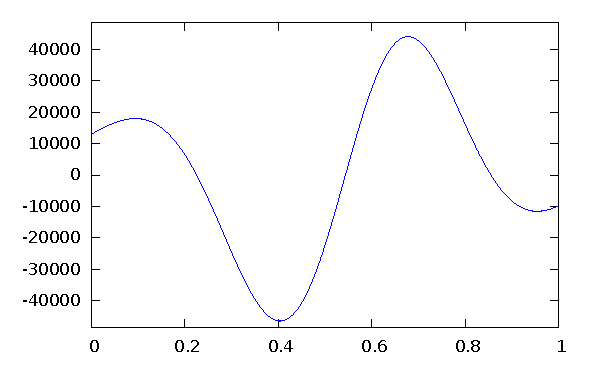
\includegraphics[scale=0.75]{figures/interpolation-polynomials2}\tabularnewline
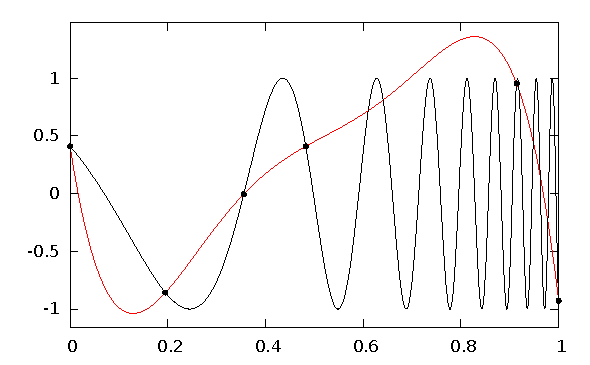
\includegraphics[scale=0.75]{figures/interpolation-polynomials3} & 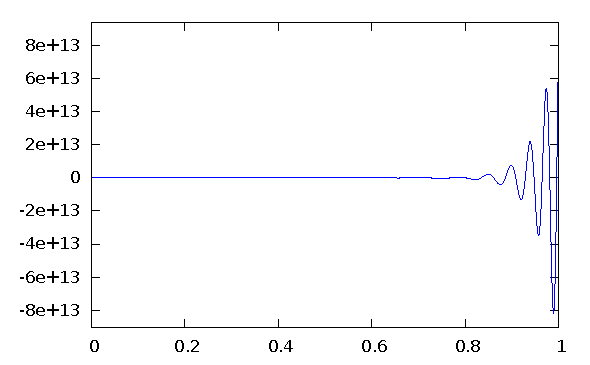
\includegraphics[scale=0.75]{figures/interpolation-polynomials4}\tabularnewline
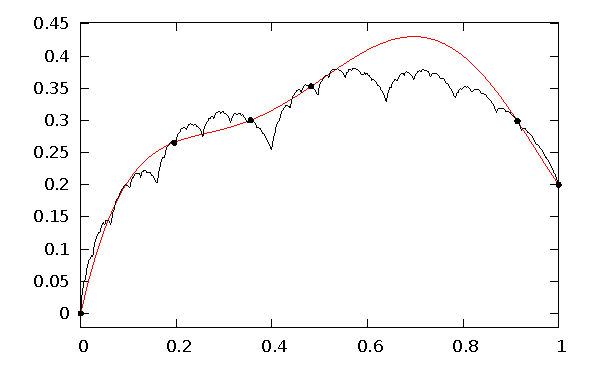
\includegraphics[scale=0.75]{figures/interpolation-polynomials5} & 
\includegraphics[scale=0.75]{figures/undefined}\tabularnewline
\end{tabular}
\end{figure}
 memperlihatkan polinom interpolasi untuk tiga fungsi yang berbeda.
Koordinat $x$ dari titik-titik yang ditentukan sama untuk setiap
polinom interpolasi. Koordinat $x$ tersebut adalah 
\[
0,.1951846177977887,.3554400571592862,.4823905248516196,.9138095996128959,\mbox{ dan }1.
\]
Empat bilangan di antara 0 dan 1 dipilih dengan generator bilangan
acak. Hanya pada kasus pertama polinom interpolasi sangat menyerupai
fungsinya. Turunan keenam $f$ membantu menjelaskan alasannya. 

Suku galat kita, 
\[
\frac{f^{(6)}(\xi)}{6!}(x-x_{0})(x-x_{1})\cdots(x-x_{5})
\]
menyiratkan bahwa turunan keenam $f$ dan polinom $h(x)=\frac{(x-x_{0})(x-x_{1})\cdots(x-x_{5})}{6!}$
menentukan seberapa besar perbedaan antara $f$ dan $L_{6}$. Dengan
membatasi $\left|f^{(6)}\right|$ dan $\left|h\right|$ pada selang
$[0,1]$, kita dapat memperoleh batas bagi selisih antara $f$ dan
$L_{6}$. Grafik $f^{(6)}$ ditampilkan pada Gambar \ref{fig:Three-interpolating-functions.}.
Grafik $h$ adalah

\begin{center}
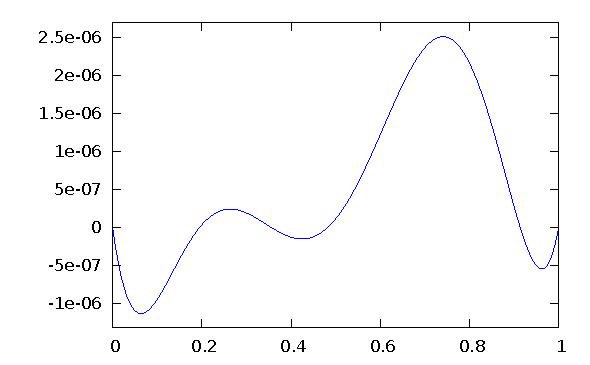
\includegraphics{figures/interpolation-polynomials6}
\par\end{center}

\noindent sehingga $\max_{x\in[0,1]}|h(x)|$ terjadi di sekitar $0.75$.
Kita dapat menerapkan metode pencarian akar pada $h'$ untuk menemukan
bahwa maksimum $|h|$ kira-kira $h(.7409254943919)\approx2.506891519629(10)^{-6}$,
suatu bilangan yang relatif kecil. Di sisi lain, untuk $f(x)=e^{\sin\left((x+1)^{2}\right)}$,
kita memperoleh $\max_{x\in[0,1]}\left|f^{(6)}(x)\right|\approx f^{(6)}(.6777170541644)\approx44013.74605321$,
suatu bilangan yang relatif besar. Hasil kali keduanya,
\[
\max_{x\in[0,1]}|h(x)|\cdot\max_{x\in[0,1]}\left|f^{(6)}(x)\right|\approx.11,
\]
memberikan batas galat. Jarak mutlak terbesar antara $L_{6}$ dan
$f$ pada selang $[0,1]$ tidak mungkin melebihi $0.11$, suatu bilangan
yang relatif kecil. Galat sebenarnya jauh lebih kecil sehingga hampir
tidak terlihat pada grafik kiri atas Gambar \ref{fig:Three-interpolating-functions.}.

Untuk $f(x)=\sin\left(e^{(x+1)^{2}}\right)$, kita memperoleh $\max_{x\in[0,1]}\left|f^{(6)}(x)\right|\approx f^{(6)}(1)\approx8.552147927657737(10)^{13}$,
suatu bilangan yang relatif besar. Kali ini hasil kalinya,
\[
\max_{x\in[0,1]}|h(x)|\cdot\max_{x\in[0,1]}\left|f^{(6)}(x)\right|\approx2.1439307114460004(10)^{8},
\]
merupakan bilangan yang sangat besar dibandingkan dengan nilai $f$.
Jadi, batas galat teoretis tidak meramalkan hasil yang baik bagi interpolasi
ini. Bahkan, batas itu menunjukkan bahwa interpolasinya dapat jauh,
jauh lebih buruk!$L_{6}$ mungkin berbeda dari $f$ sebesar lebih
dari dua juta; hal ini patut dikhawatirkan karena $f$ bernilai antara
$-1$ dan $1$. Hampiran yang meleset bahkan sebesar $1$ sama sekali
tidak berguna untuk fungsi $f$ ini. Dalam keadaan ini, kita tidak
perlu terkejut bahwa $L_{6}$ bukan hampiran yang baik terhadap $f$
karena suku galatnya dapat sangat besar. Meskipun demikian, metodenya
tetap sah. Kegagalan menghampiri $f$ dengan baik bukanlah kelemahan
metode, melainkan kekeliruan dalam penerapannya. Jika kita benar-benar
ingin menghampiri $f$ dengan baik, kita perlu memilih himpunan titik
interpolasi yang berbeda.

Untuk fungsi fraktal di kiri bawah Gambar \ref{fig:Three-interpolating-functions.},
taksiran galat kita sama sekali tidak relevan. Turunan keenam $f$
tidak ada. Bahkan, turunan pertama $f$ pun tidak ada. Kita tidak
dapat menaksir galat selain dengan melihat grafik. Dan seperti terlihat,
$L_{6}$ kembali menjadi hampiran yang sangat buruk terhadap $f$.
Sekali lagi, kegagalan itu bukanlah kelemahan metode, melainkan kekeliruan
penerapannya. Menghampiri fungsi dengan polinom interpolasi mengandaikan
bahwa fungsi tersebut mempunyai cukup banyak turunan.

\noindent\begin{digression}{Polinom Bernstein}\index{polinom Bernstein}

\noindent Misalkan $f$ adalah fungsi kontinu pada selang $[0,1]$,
dan definisikan polinom
\[
B_{n}(x)=\sum_{\nu=0}^{n}\begin{pmatrix}n\\
\nu
\end{pmatrix}f\left(\frac{\nu}{n}\right)x^{\nu}(1-x)^{n-\nu},\quad n=1,2,3,\ldots
\]
Maka 
\[
\lim_{n\to\infty}B_{n}(x)=f(x)
\]
secara seragam. Artinya, $\lim_{n\to\infty}\max\{|B_{n}(x)-f(x)|:x\in[0,1]\}=0$.
Polinom $B_{n}$ disebut polinom Bernstein. Di bawah ini ditampilkan
$B_{4}$, $B_{20}$, $B_{100}$, dan $B_{500}$ untuk fungsi fraktal
pada Gambar \ref{fig:Three-interpolating-functions.}.

\begin{center}
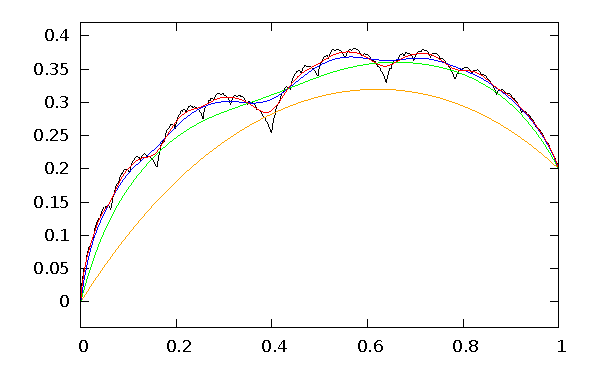
\includegraphics{figures/interpolation-polynomials7}
\par\end{center}

\noindent\end{digression}

\subsection{Penerapan polinom interpolasi}

Sekali lagi kita menghubungkan materi bab sebelumnya dengan bab ini.
Metode sekan sebenarnya merupakan penerapan polinom interpolasi pada
pencarian akar. Garis sekan yang kemiringannya digunakan untuk menghitung
suatu iterasi dapat dipandang sebagai garis interpolasi! Garis itu
melalui dua titik pada $g$. Karena itu, garis tersebut merupakan
hampiran terhadap $g$.

Dengan sudut pandang ini, kita dapat menggeneralisasi metode tersebut
dengan menggunakan turunan polinom interpolasi berderajat lebih tinggi
untuk menghampiri $g'$ pada setiap langkah. Metode umum ini, yang
akan kita sebut metode Sidi berderajat $k$ \cite{sidi},\index{metode Sidi}\index{metode!Sidi|see{metode Sidi}}
diringkas oleh rumus 
\[
x_{n+1}=x_{n}-\frac{g(x_{n})}{p'_{n,k}(x_{n})}
\]
 dengan $p_{n,k}$ sebagai polinom interpolasi yang melalui titik-titik
\[
(x_{n},g(x_{n})),(x_{n-1},g(x_{n-1})),\ldots,(x_{n-k},g(x_{n-k})).
\]
Untuk $k=1$, metode ini tepat sama dengan metode sekan. Untuk $k=2$,
metode ini menggunakan parabola yang sama dengan metode M�ller, tetapi
dengan cara yang berbeda. Pada metode M�ller, iterasi berikutnya diperoleh
dengan mencari akar polinom interpolasi. Pada metode ini, iterasi
berikutnya diperoleh dengan mencari akar garis singgung pada polinom
interpolasi.

Ketika $k$ bertambah, diperlukan lebih banyak nilai awal, tetapi
sebagai imbalannya orde kekonvergenan meningkat. Dengan $\alpha_{k}$
sebagai orde kekonvergenan metode Sidi berderajat $k$, kita mempunyai
$\alpha_{1}=\frac{1+\sqrt{5}}{2}\approx1.618$, yaitu orde kekonvergenan
metode sekan, dan
\[
\alpha_{2}\approx1.839,\ \alpha_{3}\approx1.928,\ \alpha_{4}\approx1.966.
\]
Untuk setiap $k$, metode Sidi mempunyai orde kekonvergenan kurang
dari 2 (orde kekonvergenan metode Newton), tetapi mendekati 2 ketika
$k$ bertambah.

Pada titik ini, Anda mungkin bertanya-tanya seberapa praktis metode
tersebut. Lagi pula, menghitung polinom interpolasi Lagrange baru
dan mengevaluasi turunannya pada setiap langkah dapat menjadi proses
yang merepotkan. Kita akan membahas persoalan ini pada bagian berikutnya.

\subsection{Metode Neville\index{metode Neville}\index{metode!Neville|see{metode Neville}}}

\label{NevillesMethodDiscussion}Bagi manusia, bentuk Lagrange dari
polinom interpolasi sudah sangat praktis. Dengan sedikit ketelitian
dan kesabaran, polinom semacam itu dapat dituliskan bahkan tanpa bantuan
kalkulator. Namun, menambahkan titik interpolasi dan mengevaluasi
polinom pada titik yang bukan titik interpolasi dapat menjadi pekerjaan
yang merepotkan. Tinjau contoh sederhana: polinom yang menginterpolasi
$f(x)=e^{x}$ pada $x=0,1,2$:
\begin{eqnarray*}
L_{2}(x) & = & \frac{(x-1)(x-2)}{(0-1)(0-2)}e^{0}+\frac{(x-0)(x-2)}{(1-0)(1-2)}e^{1}+\frac{(x-0)(x-1)}{(2-0)(2-1)}e^{2}\\
 & = & \frac{(x-1)(x-2)}{2}+\frac{x(x-2)}{-1}e+\frac{x(x-1)}{2}e^{2}.
\end{eqnarray*}
Sebagai contoh, mengevaluasi $L_{2}(1.5)$ memerlukan salah satu dari
dua cara berikut:
\begin{enumerate}
\item menghitung nilai ketiga suku secara terpisah, yang masing-masing merupakan
polinom kuadrat, lalu menjumlahkannya:
\begin{eqnarray*}
L_{2}(1.5) & = & \frac{(1.5-1)(1.5-2)}{2}+\frac{1.5(1.5-2)}{-1}e+\frac{1.5(1.5-1)}{2}e^{2}\\
 & = & -.125+.75e+.375e^{2}\\
 & \approx & 4.684607408443278
\end{eqnarray*}
atau
\item menjabarkan $L_{2}$ ke bentuk polinom biasa, lalu mengevaluasinya:
\begin{eqnarray*}
L_{2}(x) & = & \frac{(x-1)(x-2)}{2}+\frac{x(x-2)}{-1}e+\frac{x(x-1)}{2}e^{2}\\
 & = & \frac{1}{2}(x^{2}-3x+2)-e(x^{2}-2x)+\frac{e^{2}}{2}(x^{2}-x)\\
 & = & \left(\frac{1}{2}-e+\frac{e^{2}}{2}\right)x^{2}+\left(-\frac{3}{2}+2e-\frac{e^{2}}{2}\right)x+1\\
 & \approx & 1.47624622100628x^{2}+0.242035607452765x+1
\end{eqnarray*}
sehingga $L_{2}(1.5)\approx1.47624622100628(1.5)^{2}+0.242035607452765(1.5)+1=4.684607408443277$.
\end{enumerate}
Metode 2 lebih baik jika Anda hendak mengevaluasi pada lebih banyak
titik, sedangkan metode 1 lebih baik jika Anda berencana menambah
titik interpolasi. Namun, kedua metode tersebut tidak terlalu praktis.
Yang bahkan lebih merepotkan daripada mengevaluasi polinom adalah
menambahkan satu lagi titik interpolasi. Hasil perhitungan sebelumnya
hanya sedikit membantu. Kita bahkan belum membahas sulitnya menulis
program komputer untuk mengotomatiskan perhitungan. Metode Neville
dapat mengatasi keterbatasan ini ketika nilai polinom pada suatu titik
tertentu diperlukan.

Metode Neville didasarkan pada pengamatan bahwa polinom interpolasi
dapat dikonstruksi secara rekursif. Misalkan $P_{k,l}$ adalah polinom
berderajat paling tinggi $l$ yang menginterpolasi data
\[
(x_{k},f(x_{k})),(x_{k+1},f(x_{k+1})),\ldots,(x_{k+l},f(x_{k+l})).
\]
Maka, menurut definisi, $P_{0,n}$ adalah polinom berderajat paling
tinggi $n$ yang menginterpolasi data 
\[
(x_{0},f(x_{0})),(x_{1},f(x_{1})),\ldots,(x_{n},f(x_{n})).
\]
Selain itu, polinom ini dapat dihitung menggunakan rumus rekursif
\begin{eqnarray}
P_{i,m+1}(x) & = & \frac{(x-x_{i})P_{i+1,m}(x)-(x-x_{i+m+1})P_{i,m}(x)}{x_{i+m+1}-x_{i}}\nonumber \\
P_{i,0}(x) & = & f(x_{i}),\qquad i=0,\ldots,n.\label{eq:NevillesRecursion}
\end{eqnarray}
Pernyataan ini dapat diperiksa dengan memperhatikan lima hal berikut:\label{shellProofOfNevillesMethod}
\begin{enumerate}
\item $P_{i,0}$ adalah polinom derajat 0 yang menginterpolasi satu datum
$(x_{i},f(x_{i}))$.
\item $P_{i,m}$ dan $P_{i+1,m}$ adalah polinom-polinom berderajat paling
tinggi $m$, sehingga $P_{i,m+1}$ adalah polinom berderajat paling
tinggi $m+1$.
\item ${\displaystyle P_{i,m+1}(x_{i})=\frac{-(x_{i}-x_{i+m+1})P_{i,m}(x_{i})}{x_{i+m+1}-x_{i}}=P_{i,m}(x_{i})=f(x_{i})}$.
\item Untuk setiap $j=i+1,\ldots,i+m$,
\begin{eqnarray*}
P_{i,m+1}(x_{j}) & = & \frac{(x_{j}-x_{i})P_{i+1,m}(x_{j})-(x_{j}-x_{i+m+1})P_{i,m}(x_{j})}{x_{i+m+1}-x_{i}}\\
 & = & \frac{(x_{j}-x_{i})f(x_{j})-(x_{j}-x_{i+m+1})f(x_{j})}{x_{i+m+1}-x_{i}}\\
 & = & \frac{f(x_{j})\left[(x_{j}-x_{i})-(x_{j}-x_{i+m+1})\right]}{x_{i+m+1}-x_{i}}\\
 & = & f(x_{j}).
\end{eqnarray*}
\item ${\displaystyle P_{i,m+1}(x_{i+m+1})=\frac{(x_{i+m+1}-x_{i})P_{i+1,m}(x_{i+m+1})}{x_{i+m+1}-x_{i}}=P_{i+1,m}(x_{i+m+1})=f(x_{i+m+1})}$.
\end{enumerate}
Bukti ketat dengan induksi terhadap $m$, yang diminta dalam latihan,
dapat disusun dengan mengikuti catatan ini. Butir 1 dan 2 menunjukkan
bahwa $P_{k,l}$ berderajat paling tinggi $l$. Butir 3 hingga 5 menunjukkan
bahwa $P_{k,l}$ menginterpolasi titik-titik $(x_{k},f(x_{k})),(x_{k+1},f(x_{k+1})),\ldots,(x_{k+l},f(x_{k+l}))$.
Rumus \ref{eq:NevillesRecursion} merangkum metode Neville secara
ringkas.

Walaupun metode Neville (rumus \ref{eq:NevillesRecursion}) dapat
digunakan untuk mencari rumus polinom interpolasi seperti
\begin{eqnarray*}
P_{0,1}(x) & = & \frac{(x-x_{0})P_{1,0}(x)-(x-x_{1})P_{0,0}(x)}{x_{1}-x_{0}}\\
 & = & \frac{x-x_{1}}{x_{0}-x_{1}}f(x_{0})+\frac{x-x_{0}}{x_{1}-x_{0}}f(x_{1}),
\end{eqnarray*}
metode ini biasanya digunakan untuk mencari nilai polinom interpolasi
pada suatu titik tertentu. Sebelumnya kita memperoleh $L_{2}(1.5)=4.684607408443277$
untuk polinom $L_{2}(x)$ yang menginterpolasi $f(x)=e^{x}$ pada
$x=0,1,2$. Sekarang kita akan mencari nilai ini menggunakan metode
Neville. $P_{0,0}(1.5)=f(0)=1$, $P_{1,0}(1.5)=f(1)\approx2.718281828459045$,
dan $P_{2,0}(1.5)=f(2)\approx7.38905609893065$. Jadi
\begin{eqnarray*}
P_{0,1}(1.5) & = & \frac{(1.5-x_{0})P_{1,0}(1.5)-(1.5-x_{1})P_{0,0}(1.5)}{x_{1}-x_{0}}\\
 &  & =\frac{(1.5-0)(2.718281828459045)-(1.5-1)(1)}{1-0}\\
 &  & \approx3.577422742688568\\
P_{1,1}(1.5) & = & \frac{(1.5-x_{1})P_{2,0}(1.5)-(1.5-x_{2})P_{1,0}(1.5)}{x_{2}-x_{1}}\\
 & = & \frac{(1.5-1)(7.38905609893065)-(1.5-2)(2.718281828459045)}{2-1}\\
 & \approx & 5.053668963694848\\
P_{0,2}(1.5) & = & \frac{(1.5-x_{0})P_{1,1}(1.5)-(1.5-x_{2})P_{0,1}(1.5)}{x_{2}-x_{0}}\\
 & = & \frac{(1.5-0)(5.053668963694848)-(1.5-2)(3.577422742688568)}{2-0}\\
 & \approx & 4.684607408443278.
\end{eqnarray*}
Menyusun perhitungan dalam tabel dapat memudahkan kita memahami rekursi
dan membayangkan cara mengotomatiskan proses ini. Tabel \ref{tab:NevillesMethodExample}
\begin{table}
\hrule \caption{\label{tab:NevillesMethodExample}Contoh metode Neville: menghitung
$P_{0,2}(1.5)$.}

\centering{}\medskip{}
\begin{tabular}{cccc}
$x_{i}$ & $P_{i,0}=f(x_{i})$ & $P_{i,1}$ & $P_{i,2}$\tabularnewline
\hline 
$0$ & $1$ & $3.577422742688568$ & $4.684607408443278$\tabularnewline
$1$ & $2.718281828459045$ & $5.053668963694848$ & \tabularnewline
$2$ & $7.38905609893065$ &  & \tabularnewline
\end{tabular}\medskip{}
\hrule 
\end{table}
 menampilkan tabulasi tersebut. Bagi manusia, menggunakan rumus rekursif
ini mungkin lebih sulit daripada menghitungnya secara langsung. Namun,
bagi komputer, rekursi jauh lebih cepat dan sederhana, sebagaimana
terlihat dari kode semu. 

\begin{pseudocode} \index{metode Neville!kode semu}\label{NevillesMethodPseudoCode}
\begin{description}
\item [{Asumsi:}] $P_{n}(x)$ adalah polinom berderajat paling tinggi $n$
yang menginterpolasi data
\[
(x_{0},f(x_{0})),(x_{1},f(x_{1})),\ldots,(x_{n},f(x_{n}))
\]
dan nilai $P_{n}(\hat{x})$ hendak dicari.
\item [{Masukan:}] Nilai $\hat{x}$; absis $x_{0},x_{1},\ldots,x_{n}$;
ordinat $f(x_{0}),f(x_{1}),\ldots,f(x_{n})$.
\item [{Langkah~1:}] Untuk $i=0\ldots n$ lakukan Langkah 2:

\begin{description}
\item [{Langkah~2:}] Tetapkan $P_{i,0}=f(x_{i})$;
\end{description}
\item [{Langkah~3:}] Untuk $j=1\ldots n$ lakukan Langkah 4--5:

\begin{description}
\item [{Langkah~4:}] Untuk $i=0\ldots n-j$ lakukan Langkah 5:

\begin{description}
\item [{Langkah~5:}] Tetapkan $P_{i,,j}=\frac{(\hat{x}-x_{i})P_{i+1,j-1}(\hat{x}-x_{i+j})P_{i,j-1}}{x_{i+j}-x_{i}}$
\end{description}
\end{description}
\item [{Keluaran:}] Tabel nilai, $P$. $P_{0,n}$ memuat nilai yang dicari,
$L_{n}(\hat{x})$.
\end{description}
\end{pseudocode}  

\subsection{Keunikan}

Ada beberapa seluk-beluk yang sejauh ini belum kita bahas. Ketika
memperkenalkan bentuk Lagrange, kita begitu saja menyatakan ``$L_{n}$
disebut \textit{bentuk Lagrange} dari $P_{n}$'', yang menyiratkan
bahwa bentuk Lagrange menghasilkan polinom interpolasi \textit{berderajat
terendah} (karena $P_{n}$ memang didefinisikan demikian)! Fakta ini
sama sekali tidak langsung terlihat. Meskipun demikian, kita melanjutkan
seolah-olah sudah jelas bahwa $L_{n}$ dan $P_{n}$ merupakan polinom
yang sama. Lebih buruk lagi, ketika membahas metode Neville, kita
menghitung $P_{0,2}(1.5)$ dan membandingkannya dengan $L_{2}(1.5)$
yang diperoleh sebelumnya, seolah-olah keduanya memang harus sama;
sekali lagi, seolah-olah sudah pasti bahwa $P_{0,2}$ dan $L_{2}$
merupakan polinom yang sama. Hasil berikut menunjukkan bahwa kepercayaan
kita tanpa bukti bahwa $P_{n}$, $L_{n}$, dan $P_{0,n}$ sekadar
nama-nama berbeda bagi objek yang sama ternyata tidak keliru (karena
semuanya menginterpolasi data yang sama dan berderajat paling tinggi
$n$).
\begin{thm}
\label{thm:interpolatingPolynomialUniqueness}Polinom $P_{n}$ berderajat
terendah yang menginterpolasi data $(x_{0},y_{0}),(x_{1},y_{1}),\ldots,(x_{n},y_{n})$
ada dan bersifat unik. Selain itu, setiap polinom interpolasi berderajat
paling tinggi $n$ sama dengan $P_{n}$.
\end{thm}

\begin{proof}
Berdasarkan konstruksinya, $L_{n}$ menginterpolasi data. Selain itu,
$L_{n}$ berderajat paling tinggi $n$ karena polinom ini merupakan
jumlah dari polinom-polinom $p_{i}$ yang masing-masing berderajat
tepat $n$. Dengan demikian, $P_{n}$ ada dan berderajat paling tinggi
$n$ {[}pada titik ini, harus kita akui bahwa derajat $P_{n}$ mungkin
lebih rendah daripada derajat $L_{n}${]}. Sekarang misalkan $q$
adalah sembarang polinom yang menginterpolasi $(x_{0},y_{0}),(x_{1},y_{1}),\ldots,(x_{n},y_{n})$
dan berderajat $n$ atau kurang. Maka polinom $f=P_{n}-q$ juga berderajat
$n$ atau kurang. Selain itu, $f(x_{i})=P_{n}(x_{i})-q(x_{i})=y_{i}-y_{i}=0$
untuk setiap $i-0,\ldots,n$. Dengan demikian, $f$ mempunyai $n+1$
akar. Satu-satunya cara $f$ dapat mempunyai $n+1$ akar sekaligus
berderajat $n$ atau kurang adalah jika $f$ identik dengan 0. Oleh
karena itu, $f(x)=P_{n}(x)-q(x)=0$, sehingga $P_{n}(x)=q(x)$ untuk
setiap $x$.
\end{proof}

\subsection{Octave}

\label{NevillesMethodOctaveCode}\index{metode Neville!kode Octave}Indeks
yang disajikan dalam kode semu didasarkan pada pengindeksan yang dimulai
dari 0, seperti dalam uraian matematis. Namun, di Octave indeks tidak
dapat bernilai 0. Indeks selalu berupa bilangan bulat positif. Sedikit
penyesuaian indeks diperlukan untuk mengakomodasi perbedaan ini.

\noindent\begin{verbatim}
%%%%%%%%%%%%%%%%%%%%%%%%%%%%%%%%%%%%%%%%%%%%%%%%%%%%%%%%%%%%%%%%
% Written by Leon Brin                        11 December 2020 %
% Purpose: This function implements Neville's method for       %
%        computing the value P(xhat) of the interpolating      %
%        polynomial P passing through the data (x(1),y(1)),    %
%        (x(2),y(2)),...,(x(n),y(n)).                          %
% INPUT: value xhat; array x of abscissas; array y of          %
%        ordinates.                                            %
% OUTPUT: table of values Q; Q(1,n)=P(xhat).                   %
%%%%%%%%%%%%%%%%%%%%%%%%%%%%%%%%%%%%%%%%%%%%%%%%%%%%%%%%%%%%%%%%
function Q = nevilles(xhat,x,y)
  n=length(x);
  for i=1:n
    Q(i,1)=y(i);
  end%for
  for j=2:n
    for i=1:n+1-j
      Q(i,j)=((xhat-x(i))*Q(i+1,j-1)-(xhat-x(i+j-1))*Q(i,j-1))/(x(i+j-1)-x(i));
    end%for
  end%for
end%function 
\end{verbatim}\texttt{nevilles.m} dapat diunduh di \href{http://lqbrin.github.io/tea-time-numerical/ancillaries.html}{situs pendamping}.

\subsection{Konsep Utama}
\begin{description}
\item [{Fungsi~interpolasi:}] \index{fungsi interpolasi}Fungsi yang grafiknya
harus melalui sekumpulan titik yang ditentukan.
\item [{Polinom~interpolasi:}] \index{polinom interpolasi}Polinom yang
grafiknya harus melalui sekumpulan titik yang ditentukan.  
\item [{Polinom~interpolasi~yang~berderajat~terendah:}] Polinom berderajat
terendah yang menginterpolasi sekumpulan $n+1$ titik data bersifat
unik. Kita menyatakan polinom ini dengan $P_{n}$.
\item [{Polinom~interpolasi~dengan~derajat~paling~tinggi~$n$:}] Polinom
yang menginterpolasi $n+1$ titik berbeda berderajat paling tinggi
$n$ dan sama dengan polinom berderajat terendah yang menginterpolasi
titik-titik tersebut.
\item [{Teorema~Rolle~yang}] Diperumum: \index{Teorema!Rolle yang Diperumum}Misalkan
$f$ mempunyai $n$ turunan pada $(a,b)$ dan $f,f',f'',\ldots,f^{(n-1)}$
semuanya kontinu pada $[x_{0},x_{n}]$. Jika $f(x_{0})=f(x_{1})=\cdots=f(x_{n})$
untuk suatu $x_{0}<x_{1}<\cdots<x_{n}$, maka terdapat $\xi\in(a,b)$
sedemikian sehingga $f^{(n)}(\xi)=0$.
\item [{Bentuk~Lagrange~dari~suatu~polinom~interpolasi:}] \index{bentuk Lagrange}Bentuk
Lagrange, $L_{n}$, dari polinom berderajat paling tinggi $n$ yang
menginterpolasi titik-titik $(x_{0},y_{0}),(x_{1},y_{1}),\ldots,(x_{n},y_{n})$
diberikan oleh rumus
\[
L_{n}(x)=\sum_{i=0}^{n}\frac{p_{i}(x)}{p_{i}(x_{i})}y_{i},
\]
dengan ${\displaystyle p_{i}(x)=\prod_{\substack{j=0\\
j\neq i
}
}^{n}(x-x_{j})=(x-x_{0})\cdots(x-x_{i-1})(x-x_{i+1})\cdots(x-x_{n})}$.
\item [{Galat~interpolasi:}] Untuk $P_{n}$, polinom interpolasi berderajat
terendah yang melalui $n+1$ titik $(x_{0},y_{0}),(x_{1},y_{1}),\ldots,(x_{n},y_{n})$,
terdapat $\xi_{x}\in(a,b)$ sedemikian sehingga
\[
f(x)-P_{n}(x)=\frac{f^{(n+1)}(\xi_{x})}{(n+1)!}(x-x_{0})(x-x_{1})\cdots(x-x_{n}),
\]
dengan asumsi $f$ mempunyai $n+1$ turunan pada $(a,b)$ dan $f,f',f'',\ldots,f^{(n)}$
semuanya kontinu pada $[a,b]$, dengan $a=\min(x_{0},\ldots,x_{n},x)$
dan $b=\max(x_{0},\ldots,x_{n},x)$.
\item [{Metode~Sidi:}] \index{metode Sidi}Metode pencarian akar yang
diringkas oleh rumus 
\[
x_{n+1}=x_{n}-\frac{f(x_{n})}{p'_{n,k}(x_{n})}
\]
dengan $p_{n,k}$ sebagai polinom interpolasi yang melalui titik-titik
\[
(x_{n},f(x_{n})),(x_{n-1},f(x_{n-1})),\ldots,(x_{n-k},f(x_{n-k})).
\]
\item [{Metode~Neville:}] \index{metode Neville}Metode untuk menghitung
polinom interpolasi berderajat terendah atau nilai-nilainya berdasarkan
relasi rekursif
\begin{eqnarray*}
P_{i,m+1}(x) & = & \frac{(x-x_{i})P_{i+1,m}(x)-(x-x_{i+m+1})P_{i,m}(x)}{x_{i+m+1}-x_{i}}\\
P_{i,0}(x) & = & f(x_{i})
\end{eqnarray*}
dengan $P_{k,l}$ sebagai polinom berderajat terendah yang menginterpolasi
data
\[
(x_{k},f(x_{k})),(x_{k+1},f(x_{k+1})),\ldots,(x_{k+l},f(x_{k+l})).
\]
\end{description}
\startexercises 

\subsection{Latihan}
\begin{enumerate}
\item Tuliskan polinom interpolasi Lagrange yang melalui $(1,2)$, $(1.5,-0.83)$,
dan $(2.11,-1)$.
\item Carilah polinom yang melalui keempat titik
\[
(0,0),\ (1,2),\ (4,-3),\mbox{ dan }(10,-1).
\]
\item \label{exc:interpolation-lagrange}Konstruksikan polinom Lagrange
(berderajat paling tinggi dua) yang menginterpolasi data berikut.

\begin{enumerate}
\item $(1,1)$, $(2,1)$, dan $(3,2)$
\item $(0,10)$, $(30,58)$, $(1029,-32)$
\item \label{exc:interpolation-lagrange-8}$(-10,10)$, $(20,58)$, $(1019,-32)$ \hasasolution 
\item $\ $

\begin{center}
\begin{tabular}{c|c}
$x$ & $f(x)$\tabularnewline
\hline 
$5$ & $15$\tabularnewline
$200$ & $2$\tabularnewline
$10$ & $15$\tabularnewline
\end{tabular}
\par\end{center}
\item $\ $

\begin{center}
\begin{tabular}{c|c}
$x$ & $f(x)$\tabularnewline
\hline 
$-5$ & $15$\tabularnewline
$-2$ & $2$\tabularnewline
$3$ & $15$\tabularnewline
\end{tabular}
\par\end{center}
\end{enumerate}
\item \label{exc:interpolation-lagrange-7}Misalkan data pada soal \ref{exc:interpolation-lagrange}
berasal dari suatu fungsi $f$ yang dapat didiferensialkan secukupnya.
Gunakan polinom interpolasi yang Anda peroleh pada soal \ref{exc:interpolation-lagrange}
untuk menghampiri $f(1.3)$. \haspartwithsolution 
\item \label{exc:interpolation-lagrange-2}Carilah hampiran pada soal \ref{exc:interpolation-lagrange-7}
menggunakan metode Neville. \haspartwithsolution 
\item Diberikan data berikut untuk $f(x)$, hampiri $f(0.3)$ menggunakan
polinom interpolasi berderajat paling tinggi

\begin{enumerate}
\item 1
\item 2
\item 3
\end{enumerate}
\begin{center}
\begin{tabular}{c|cccc}
$x$ & $0$ & $1$ & $2$ & $3$\tabularnewline
\hline 
$f(x)$ & $0.8$ & $0.7$ & $0.75$ & $0.5$\tabularnewline
\end{tabular}
\par\end{center}
\item \label{exc:interpolation-lagrange-9}Diberikan data berikut untuk
$f(x)$, hampiri $f(3)$ menggunakan polinom interpolasi berderajat
paling tinggi \hasasolution 

\begin{enumerate}
\item 1
\item 2
\item 3
\end{enumerate}
\begin{center}
\begin{tabular}{c|cccc}
$x$ & $2$ & $3.5$ & $4$ & $5$\tabularnewline
\hline 
$f(x)$ & $0.8$ & $0.7$ & $0.75$ & $0.5$\tabularnewline
\end{tabular}
\par\end{center}
\item \label{exc:interpolation-lagrange-6}\octave\ Gunakan polinom interpolasi
berderajat satu, dua, dan tiga untuk menghampiri setiap nilai berikut:

\begin{enumerate}
\item $f(0.43)$ jika $f(0)=1$, $f(0.25)=1.64872$, $f(0.5)=2.71828$,
$f(0.75)=4.48169$.
\item \label{exc:interpolation-lagrange-10}$f(0.18)$ jika $f(0.1)=-0.29004986$,
$f(0.2)=-0.56079734$, $f(0.3)=-0.81401972$, $f(0.4)=-1.0526302$.
 \hasasolution 
\item \label{exc:interpolation-lagrange-11}$f(2.26)$ jika $f(1)=1.654$,
$f(1.5)=-2.569$, $f(2)=-1.329$, $f(2.5)=1.776$.  \hasasolution 
\item $f(11.26)$ jika $f(10)=-0.7865$, $f(11)=-1.2352$, $f(12)=-0.8765$,
$f(13)=0.0021$.
\end{enumerate}
\item \label{exc:interpolation-lagrange-4}Misalkan $x_{0}=1$, $x_{1}=1.25$,
dan $x_{2}=1.6$. Dengan menggunakan data pada nilai-nilai $x_{i}$,
konstruksikan polinom interpolasi berderajat paling tinggi satu dan
dua, lalu gunakan keduanya untuk menghampiri $f(1.4)$. Hitung galat
absolutnya.

\begin{enumerate}
\item \label{exc:interpolation-lagrange-12}$f(x)=\sin\pi x$ \hasasolution 
\item $f(x)=\sqrt[3]{x-1}$
\item $f(x)=e^{2x-4}$
\item $f(x)=\ln(10x)$
\end{enumerate}
\item \label{exc:interpolation-lagrange-13}Gunakan rumus \ref{eq:lagrangeInterpolatingPolynomialError}
untuk mencari batas galat teoretis bagi hampiran pada soal \ref{exc:interpolation-lagrange-4}.
Bandingkan batas tersebut dengan galat sebenarnya.  \haspartwithsolution 
\item \label{exc:interpolation-lagrange-3}Suatu polinom interpolasi Lagrange
dikonstruksi untuk fungsi $f(x)=(\sqrt{2})^{x}$ dengan menggunakan
$x_{0}=0$, $x_{1}=1$, $x_{2}=2$, $x_{3}=3$. Polinom tersebut digunakan
untuk menghampiri $f(1.5)$. Carilah batas bagi galat dalam hampiran
ini.
\item Carilah polinom yang dimaksud pada soal \ref{exc:interpolation-lagrange-3}.
Kemudian

\begin{enumerate}
\item gunakan polinom tersebut untuk menghampiri $f(1.5)$; dan
\item hitung galat sebenarnya dari hampiran ini, lalu bandingkan dengan
batas yang Anda hitung pada soal \ref{exc:interpolation-lagrange-3}.
\end{enumerate}
\item \octave\ Gunakan metode Neville untuk memperoleh hampiran pada soal
\ref{exc:interpolation-lagrange-3}.
\item Ketinggian sebuah roket model diberikan pada beberapa waktu dalam
tabel berikut. Hampiri ketinggian roket pada waktu $t=0.6$ detik
menggunakan sedikitnya dua himpunan titik yang berbeda. Jelaskan hampiran
mana yang kemungkinan paling akurat.

\begin{center}
\begin{tabular}{c|c}
Waktu (detik) & Ketinggian (kaki)\tabularnewline
\hline 
$0.53238$ & $30.0534$\tabularnewline
$0.56040$ & $32.7929$\tabularnewline
$0.58842$ & $35.4956$\tabularnewline
$0.61644$ & $38.1575$\tabularnewline
\end{tabular}
\par\end{center}
\item \label{exc:interpolation-lagrange-5}Tabel berikut merupakan hasil
penggunaan metode Neville untuk menghampiri $f(0.4)$.

\begin{center}
\begin{tabular}{lllll}
\hline 
$0$ & $1$ & $2.6$ & $P_{0,2}$ & $3.016$\tabularnewline
$0.25$ & $2$ & $P_{1,1}$ & $2.96$ & \tabularnewline
$0.5$ & $P_{2,0}$ & $2.4$ &  & \tabularnewline
$0.75$ & $8$ &  &  & \tabularnewline
\hline 
\end{tabular}
\par\end{center}

Tentukan $f(0.5)$. \hasananswer 
\item \label{exc:interpolation-lagrange-14}$L_{3}(x)=-7x^{3}+57x^{2}-134x+78$
adalah polinom interpolasi berderajat paling tinggi 3 untuk data dalam
tabel. Tentukan $\omega$.  \hasananswer 

\begin{center}
\begin{tabular}{c|cccc}
$x$ & $0.5$ & $0.8$ & $\omega$ & $1.4$\tabularnewline
\hline 
$y$ & $24.375$ & $3.696$ & $0$ & $-17.088$\tabularnewline
\end{tabular}
\par\end{center}
\item Misalkan $P_{3}(x)$ adalah polinom interpolasi untuk data $(0,0)$,
$(0.5,y)$, $(1,3)$, $(2,2)$. Tentukan $y$ jika koefisien $x^{3}$
dalam $P_{3}(x)$ adalah 6.
\item Diberikan $f(x)=\sqrt{x-x^{2}}$. Misalkan $P_{2}(x)$ adalah polinom
interpolasi pada $x_{0}=0,$ $x_{1}$, dan $x_{2}=1$. Tentukan nilai
terbesar $x_{1}$ dalam $(0,1)$ yang memenuhi $f(0.5)-P_{2}(0.5)=-0.25$.
\item \label{exc:interpolation-lagrange-1}Polinom yang menginterpolasi
$n+1$ titik tidak selalu berderajat $n$. Derajatnya paling tinggi
$n$. Buatlah grafik data $(1,1)$, $(2,3)$, $(3,5)$, dan $(4,7)$,
lalu buat dugaan tentang derajat polinom yang menginterpolasi keempat
titik tersebut. Apa yang mendasari dugaan Anda?
\item Gunakan metode Neville untuk mencari polinom yang dijelaskan pada
soal \ref{exc:interpolation-lagrange-1}. Apakah derajatnya sesuai
dengan dugaan Anda?
\item \label{exc:interpolation-lagrange-15}Misalkan
\begin{eqnarray*}
x_{j} & = & 1-\frac{1}{j+1}\quad\mbox{untuk }j=0,1,2,\ldots\\
f(x) & = & 5+3x^{2018}\\
P_{n}(x) & = & \mbox{polinom interpolasi}\\
 &  & \mbox{yang melalui}\\
 &  & (x_{0},f(x_{0})),\ldots,(x_{n},f(x_{n})).
\end{eqnarray*}
Tentukan 
\[
\lim_{n\to\infty}P_{n}(1).
\]
 \hasananswer 
\item Misalkan $f(x)=e^{-x}$. Dua bilangan berbeda dipilih secara acak
dari selang $[0,1]$, sebutlah $x_{0}$ dan $x_{1}$. Kemudian titik
$(x_{0},f(x_{0}))$ dan $(x_{1},f(x_{1}))$ digunakan untuk memperoleh
hampiran interpolasi Lagrange linear bagi $f$ pada selang $[0,1]$.
Carilah suatu batas (yang berlaku untuk seluruh selang dan setiap
pasangan titik $x_{0}$ dan $x_{1}$) bagi galat penggunaan hampiran
ini.
\item Berikan bukti induktif bahwa $P_{0,n}$ adalah polinom berderajat
paling tinggi $n$ yang menginterpolasi data $(x_{0},f(x_{0})),(x_{1},f(x_{1})),\ldots,(x_{n},f(x_{n}))$.
Lihat catatan \vpageref{shellProofOfNevillesMethod}.
\end{enumerate}
\finishexercises 
